\documentclass[11pt,a4paper]{article}
\usepackage[utf8]{inputenc}
\usepackage[dvipsnames]{xcolor}
\usepackage{listings}
\usepackage{multirow}
\usepackage{color}
\usepackage{mathrsfs}
\lstset{ %
  language=R,                     % the language of the code
  basicstyle=\footnotesize,       % the size of the fonts that are used for the code
  numbers=left,                   % where to put the line-numbers
  numberstyle=\tiny\color{gray},  % the style that is used for the line-numbers
  stepnumber=1,                   % the step between two line-numbers. If it's 1, each line
                                  % will be numbered
  numbersep=5pt,                  % how far the line-numbers are from the code
  backgroundcolor=\color{white},  % choose the background color. You must add \usepackage{color}
  showspaces=false,               % show spaces adding particular underscores
  showstringspaces=false,         % underline spaces within strings
  showtabs=false,                 % show tabs within strings adding particular underscores
  frame=single,                   % adds a frame around the codehttps://da.overleaf.com/project/5e42ac84ac4e640001f94558
  rulecolor=\color{black},        % if not set, the frame-color may be changed on line-breaks within not-black text (e.g. commens (green here))
  tabsize=2,                      % sets default tabsize to 2 spaces
  captionpos=b,                   % sets the caption-position to bottom
  breaklines=true,                % sets automatic line breaking
  breakatwhitespace=false,        % sets if automatic breaks should only happen at whitespace
  title=\lstname,                 % show the filename of files included with \lstinputlisting;
                                  % also try caption instead of title
  keywordstyle=\color{blue},      % keyword style
  commentstyle=\color{ForestGreen},   % comment style
  stringstyle=\color{mauve},      % string literal style
  escapeinside={\%*}{*)},         % if you want to add a comment within your code
  morekeywords={*,...}            % if you want to add more keywords to the set
}
\usepackage{amsmath}
\usepackage{graphicx}
\usepackage{capt-of}
\usepackage{import}
\usepackage{booktabs, array}
\usepackage{siunitx}
\usepackage{tabularx}
\usepackage{dcolumn}
\usepackage{longtable}
\usepackage{amssymb}
\usepackage{arydshln}
\usepackage[english]{babel}
\usepackage{titlesec}
\graphicspath{ {pictures/} }
\addto\captionsenglish{
    \renewcommand*\contentsname{Table of Contents}
}
\usepackage{wrapfig}
\usepackage{lineno, blindtext}
\usepackage{helvet}
\usepackage{longtable}
\usepackage{fullpage}
\def\DU#1{\underline{\underline{#1}}}
\def\SU#1{\underline{#1}}
\definecolor{mygreen}{rgb}{0,0.6,0}
\usepackage{listings}

\begin{document}
\begin{titlepage} % Suppresses displaying the page number on the title page and the subsequent page counts as page 1
	\newcommand{\HRule}{\rule{\linewidth}{0.5mm}} % Defines a new command for horizontal lines, change thickness here
	
	\center % Centre everything on the page
	
	%------------------------------------------------
	%	Headings
	%------------------------------------------------
	
	\textsc{\LARGE Copenhagen Business School}\\[1.5cm] % Main heading such as the name of your university/college
	
	\textsc{\Large Statistiske Modeller}\\[0.5cm] % Major heading such as course name
	
	\textsc{\large Eksamen}\\[0.5cm] % Minor heading such as course title
	
	%------------------------------------------------
	%	Title
	%------------------------------------------------
	
	\HRule\\[0.4cm]
	
	{\huge\bfseries Statistiske Modeller}\\[0.4cm] % Title of your document
	
	\HRule\\[1.5cm]
	
	%------------------------------------------------
	%	Author(s)
	%------------------------------------------------
	
	\begin{minipage}{0.4\textwidth}
		\begin{flushleft}
			\large
			\textit{Forfattere}\\
			Lucas Johan Boesen\\ % Your name
			Christoffer Bolvig Birch\\ % Your name
			Victor Emil Skov Lundmark\\ % Your name
		\end{flushleft}
	\end{minipage}
	~
	\begin{minipage}{0.4\textwidth}
		\begin{flushright}
			\large
			\textit{Professor}\\
			\textsc{Søren Feodor Nielsen}\\
			\textsc{}\\
			\textsc{}\\% Supervisor's name
		\end{flushright}
	\end{minipage}
	
	% If you don't want a supervisor, uncomment the two lines below and comment the code above
	%{\large\textit{Author}}\\
	%John \textsc{Smith} % Your name
	
	%------------------------------------------------
	%	Date
	%------------------------------------------------
	
	\vfill\vfill\vfill % Position the date 3/4 down the remaining page
	
	{\large{December 20, 2019}} % Date, change the \today to a set date if you want to be precise
	
	%------------------------------------------------
	%	Logo
	%------------------------------------------------
	
	%\vfill\vfill
	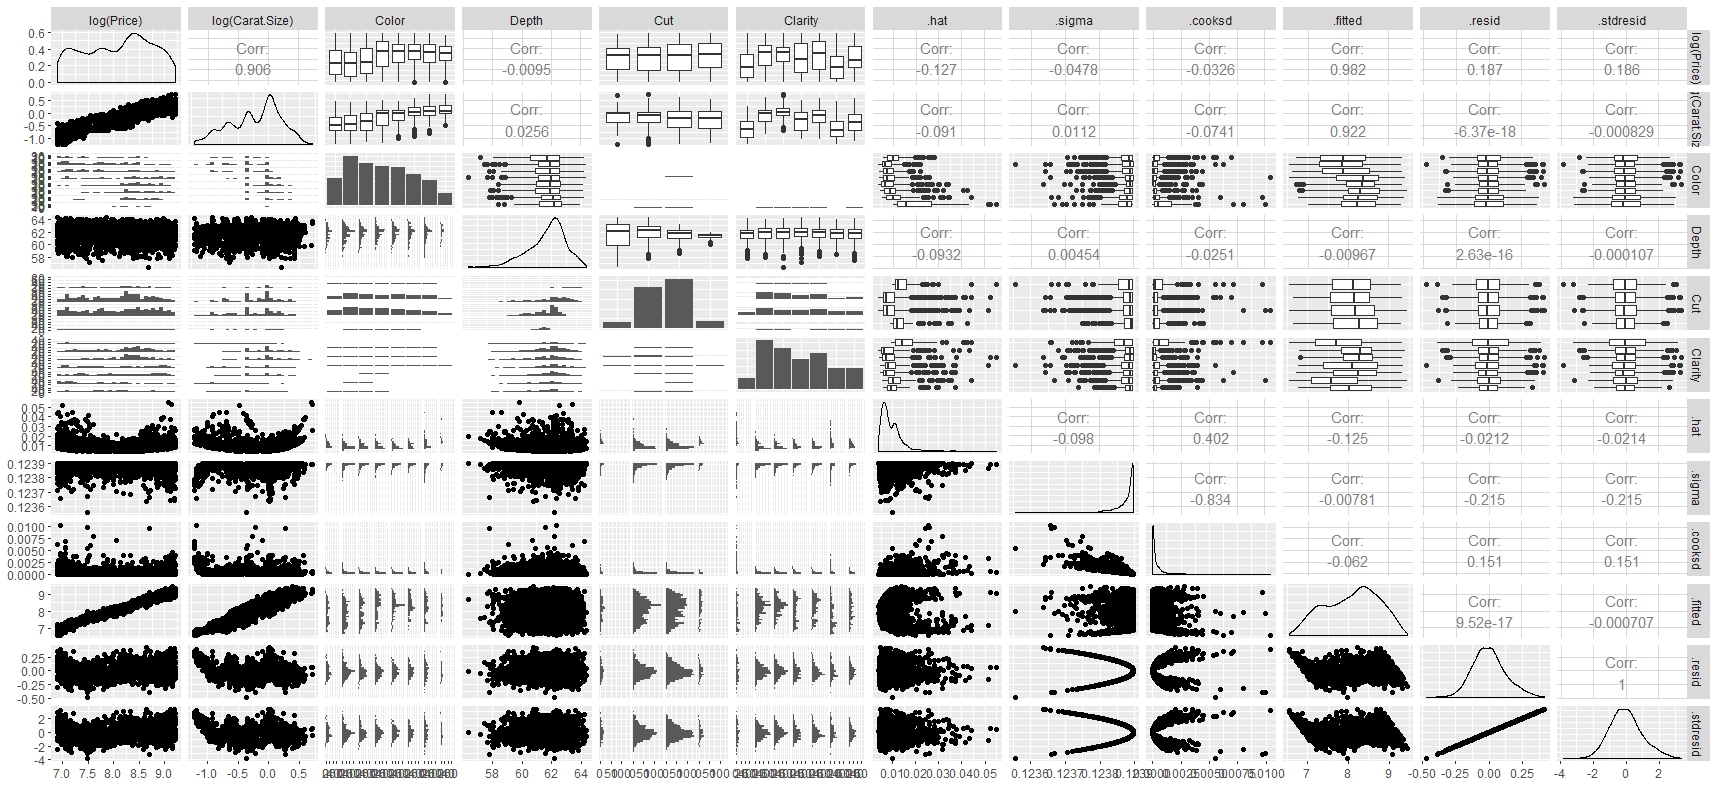
\includegraphics[width=0.8\textwidth]{kaosmuch.png}\\[1cm] % Include a department/university logo - this will require the graphicx package
	 
	%----------------------------------------------------------------------------------------
	
	\vfill % Push the date up 1/4 of the remaining page
	
\end{titlepage}
\renewcommand{\contentsname}{Indholdsfortegnelse}
\clearpage
\tableofcontents
\clearpage
\newpage
\pagenumbering{arabic}

\section{Bradley-Terry}
\subsection{Generel model}
Den generelle Bradley-Terry model, kan bruges til at beskrive sandsynligheder for parvise sammenligninger med to udfald. Sandsynligheden for at $i$ vinder over $j$ skrives op på formen: 

\begin{equation}
P(i\ vinder\ over\ j) = \pi_{ij} = \frac{\pi_i}{\pi_i+\pi_j}
\end{equation}
Hvor $\pi_{ij}$ er sandsynligheden for at $i$ vinder over $j$ og $\pi_{ij}+\pi_{ji} = 1$ skal være opfyldt, til at beskrive dette forhold anvendes $\pi_i \ og \ \pi_j$ som værende styrke parametrene for de to aktører.
Funktionen kan vises at tilhøre en eksponentiel familie, og nærmere beskrives med en logistisk fordelingsfunktion, hvilket ses ved omskrivningen af $\pi_{ij}$:\\
\begin{align*}
\pi_{ij} &= \frac{\pi_i}{\pi_i+\pi_j}=\frac{1}{1+\frac{\pi_j}{\pi_i}}=\frac{1}{1+e^{-(log(\pi_i)-log(\pi_j))}}   
\end{align*}
Herefter kan vi definere styrkeforskellen mellem de to aktører som $V = log(\pi_i)-log(\pi_j)$, hvorved vi kan omskrive funktionen til at være defineret som værende tæthedsfunktionen for en standard logistisk fordeling med lokationsparametren $\mu = 0$ og skalaparametren $s = 1$:
\begin{align*}
\frac{\partial \pi_{ij}}{\partial V} &= \frac{e^{-V}}{(e^{-V}+1)^2} = \frac{1}{(e^{V/2}+e^{-V/2})^2} = \frac{1}{4}\Big{(}\frac{2}{e^{V/2}+e^{-V/2}}\Big{)}^2 = \frac{1}{4}Sech^2(V/2)    
\end{align*}
Da differentialet nu ses at bestå af en hyperbolsk sekant, som både har den egenskab at den er symmetrisk samt i dette tilfælde opfylder $\int_{-\infty}^{\infty} \frac{1}{4}Sech^2(V/2) \; \partial V = 1$, samt at funktionen afhænger monotont af $V$, har vi at dette kan bruges som en fordelingsfunktion, hvorfor vores $\pi_{ij} \in [0,1]$. For at kunne skrive dette om til vores funktion, kan vi altså tage integralet fra $-\infty$ til $V$, som beskriver sandsynligheden for at $log(\pi_i) > log(\pi_j)$, altså at $i$ præfereres over $j$.
\begin{align*}
\pi_{ij} &= \frac{1}{1+e^{-V}} = \int_{-\infty}^{V} \frac{\partial \pi_{ij}}{\partial V} \partial V = \int_{-\infty}^{V} \frac{1}{4}Sech(V/2) \partial V    
\end{align*}
\subsection{Model som inkluderer udfaldet uafgjort}

Denne model kan ifølge P.V. Rao og L.L. Kupper "Ties in Paired-Comparison Experiments: A generalization of the Bradley-Terry model" (1967), udvides til at tage højde for den usikkerhed der kan være når man sammenligner to aktører, og dermed få sandsynligheden for $log(\pi_i)=log(\pi_j)$. Denne usikkerhed noterer vi med $\eta$, og kan beskrives som den forskel der minimum skal være mellem de to aktører for at bedømmeren kan præferere den ene over den anden. Dermed kan det siges at hvis $|V| < |\eta|$ vil sandsynligheden for at $\pi_i > \pi_j$ være tæt på 50\%, da funktionen som tidligere nævnt er symmetrisk, og mere præcist symmetrisk i anden aksen. For at få usikkerheden med, kan vi implementere den del af sandsynligheden som usikkerheden indebærer, ved at indsætte den i den øvre grænse af det bestemte integral ved:\\  
\begin{align*}
\pi_{ij} &= \int_{-\infty}^{V-\eta} \frac{1}{4}Sech(V/2) \partial V
\end{align*}
\\
Hvor $y_i=\pi_i+\epsilon_i$ kan vi nu opskrive sandsynligheden for at $i$ præfereres til $j$ som:
\begin{align*}
\pi_{ij}&=P\big{(}y_i>y_j+\eta\big{)}
\\&=P\big{(}(\pi_i-\pi_j)+(\epsilon_i-\epsilon_j)>\eta\big{)}
\\&=P\big{(}(\epsilon_i-\epsilon_j)>(\pi_i-\pi_j)+\eta\big{)}
\\&=\frac{1}{1+e^{-(log(\pi_i)-log(\pi_j)-\eta)}} 
\\&=\frac{\pi_i}{\pi_i+\theta \pi_j},\;\;\theta = e^\eta
\end{align*}
\\
Da sandsynlighederne skal summere op til 1, har vi en restsandsynlighed som beskriver udfaldet, hvor der ikke kan bestemmes om $i$ er præfereret over $j$ eller omvendt ved:
\begin{align*}
\pi_{i\cdot ij} &= P(\pi_i > \pi_j) = \frac{\pi_i}{\pi_i+\theta \pi_j}\\
\pi_{j\cdot ij} &= P(\pi_j > \pi_i) = \frac{\pi_j}{\pi_j+\theta \pi_i}\\
\pi_{0\cdot ij} &= P(\pi_j = \pi_i) = 1 - \Big{(}P(\pi_j > \pi_i) + P(\pi_i > \pi_j)\Big{)}= \frac{\pi_i \pi_j(\theta^2 -1)}{(\pi_i+\theta \pi_j)(\theta \pi_i + \pi_j)} 
\end{align*}
Hvor det selvfølgelig gælder, at $\pi_{i\cdot ij}=\pi_{i\cdot ji}$ samt at $\theta\geq1$ for at holde betingelsen \; $\pi_{i\cdot ij}\geq0,\pi_{j\cdot ij}\geq0,\pi_{0\cdot ij}\geq0$. 
\\\\
Vi kan opskrive Bradley-Terry modellen, som en multinomial fordeling: Ved først at definere antal sammenligninger $s=h(h-1)/2$ af $h$ forskellige (fx) hold eller produkter, samt antal repetitioner af disse sammenligner $r$. Observere vi $r$ repetitioner af $s$ uafhængige kategorisk variable: $$
\sum_{i<j}^s\sum_1^r\pi_{ij}^r
$$
Med de tre sandsynligheder: $\pi_{i\cdot ij},\pi_{j\cdot ij},\pi_{0\cdot ij}$
og dertilhørende udfaldstabel som værende:
$$
Y=(Y_{i\cdot ij},Y_{j\cdot ij},Y_{0\cdot ij}),\;\;\;Y_{k\cdot ij}=\sum^r1\{\pi_{k\cdot ij}\},\;\;\;\;k\in{i,j,0}
$$
vi kan nu opskrive likelihood'en:
\begin{align*}
\mathcal{L}(\pi_1,...,\pi_h,\theta) &= \prod_{i<j}\pi_{i\cdot ij}^{Y_{i\cdot ij}}\pi_{j\cdot ij}^{Y_{j\cdot ij}}\pi_{0\cdot ij}^{Y_{0\cdot ij}}\\
&= \prod_{i<j}\Big{(}\frac{\pi_i}{\pi_i+\theta\pi_j}\Big{)}^{Y_{i\cdot ij}}
\;\Big{(}\frac{\pi_j}{\pi_j+\theta\pi_i}\Big{)}^{Y_{j\cdot ij}}
\Big{(}\frac{(\theta^2-1)\pi_i \pi_j}{(\pi_i+\theta\pi_j)(\pi_j+\theta\pi_i)}\Big{)}^{Y_{0\cdot ij}}\\
\end{align*}
Vi ved at $\sum_k Y_{k\cdot ij}=1$, så vi kan omskrive $Y_{0\cdot ij}=1-Y_{i\cdot ij}-Y_{0\cdot ij}$: 
\begin{align}
\mathcal{L}(\pi_1,...,\pi_h,\theta)
&=\prod_{i<j}\Big{(}\frac{\pi_i}{\pi_i+\theta\pi_j}\Big{)}^{Y_{i\cdot ij}}
\;\Big{(}\frac{\pi_j}{\pi_j+\theta\pi_i}\Big{)}^{Y_{j\cdot ij}}
\Big{(}\frac{(\theta^2-1)\pi_i \pi_j}{(\pi_i+\theta\pi_j)(\pi_j+\theta\pi_i)}\Big{)}^{1-{Y_{i\cdot ij}}-{Y_{j\cdot ij}}}
\end{align}
hvilket giver os loglikelihooden: 
\begin{align*}
    \textit{l}(\pi,\theta)
    &=\sum_{i<j}\big{[}Y_{i\cdot ij}\;log\Big{(}\frac{\pi_i}{\pi_i+\theta\pi_j}\Big{)}
    + Y_{j\cdot ij}\;log\Big{(}\frac{\pi_j}{\pi_j+\theta\pi_i}\Big{)}
    + (1-Y_{i\cdot ij}-Y_{j\cdot ij})\;log\Big{(}\frac{(\theta^2-1)\pi_i \pi_j}{(\pi_i+\theta\pi_j)(\pi_j+\theta\pi_i)}\Big{)}\big{]}\\
    &=\sum_{i<j}\big{[}a(Y)^T\;b(\beta,\theta)+c(\beta,\theta)\big{]}\\
    \beta&=\begin{bmatrix}\beta_1\\ \beta_2\end{bmatrix}=\begin{bmatrix}log\Big{(}\frac{\pi_i}{\pi_i+\theta\pi_j}\Big{)}\\\log\Big{(}\frac{\pi_j}{\pi_j+\theta\pi_i}\Big{)} \end{bmatrix},\;\;
    a(Y)=\begin{bmatrix}Y_{i\cdot ij}\\Y_{j\cdot ij}\end{bmatrix}\;\; \\
    b(\beta,\theta)&=\begin{bmatrix}\beta_1-log(1-e^{\beta_1}-e^{\beta_2})\\\beta_2-log(1-e^{\beta_1}-e^{\beta_2})\end{bmatrix},\;\;
     c(\beta,\theta)=log(1-e^{\beta_1}-e^{\beta_2})
\end{align*}
$$
g(\beta)=-c'(\beta,\theta)^{-1}=\begin{bmatrix}\frac{1-e^{\beta_1}-e^{\beta_2}}{e^{\beta_1}}\\ \frac{1-e^{\beta_2}-e^{\beta_1}}{e^{\beta_2}}\end{bmatrix}
=
\begin{bmatrix}
\frac{\pi_i \theta + \pi_j}{\pi_j(\theta^2-1)}\\
\frac{\pi_i+\pi_j \theta}{\pi_i(\theta^2-1)}
\end{bmatrix}=\begin{bmatrix}1-\pi_{i\cdot ij}-\pi_{j\cdot ij}\\\pi_{i\cdot ij}\end{bmatrix}
$$
Vi undgår overparameterisering ved at sætte styrkeparameteret for hold r til 0. ($log(\pi_r)=0$). 
Vi kan estimere vores parametre ved brug af Newton Rhapson algoritmen:
\begin{align}
\beta^{k+1}=\beta^k+i(\beta,\theta)^{-1} \; s(\beta,\theta)
\end{align}
\begin{align}
s_y(\beta,\theta)&=\begin{bmatrix}\sum_{i<j}Y_{i\cdot ij}-\frac{(1-Y_{i\cdot ij}-Y_{j\cdot ij})e^{\beta_1}}{1-e^{\beta_1}-e^{\beta_2}}\\\sum_{i<j}Y_{i\cdot ij}-\frac{(1-Y_{i\cdot ij}-Y_{j\cdot ij})e^{\beta_2}}{1-e^{\beta_1}-e^{\beta_2}}
\end{bmatrix}\\
i(\beta,\theta)
&=\begin{bmatrix}\sum_{i<j}\frac{(1-e^{\beta_2})e^{\beta_1}(1-Y_{i\cdot ij}-Y_{j\cdot ij})}{(1-e^{\beta_1}-e^{\beta_2})^2}
&\sum_{i<j}\frac{(1-Y_{i\cdot ij}-Y_{j\cdot ij})}{(1-e^{\beta_1}-e^{\beta_2})^2}e^{\beta_1+\beta_2}
\\
\sum_{i<j}\frac{(1-Y_{i\cdot ij}-Y_{j\cdot ij})}{(1-e^{\beta_1}-e^{\beta_2})^2}e^{\beta_1+\beta_2}
&\sum_{i<j}\frac{(1-e^{\beta_1})e^{\beta_2}(1-Y_{i\cdot ij}-Y_{j\cdot ij})}{(1-e^{\beta_1}-e^{\beta_2})^2}\end{bmatrix}
\end{align}
For at kunne estimere parametrene nummerisk beskriver vi $\beta_1 \; og \; \beta_2$ ved hhv. $x_i^T\beta$ og $x_{j}^T\beta$ hvor $x_i$ er den del af designmatricen hvor hold \textit{i} indgår og $x_{j}$ er den del af designmatricen hvor hold $j$ indgår, og $\beta$ er den tilhørende parametervektor. 

\newpage
\textbf{BEMÆRK Ved score og information, har jeg differentieret mht. B1 og B2, (IKKE MHT PI(I) OG PI(J)) Jeg har også løst hvor der i loglikelihooden indsættes $\beta_1=X_i^T\beta_i$ (ja mega forvirrende med $\beta_1\neq \beta_i$) som i de er ikke det samme.Beregningerne kan findes på billedet på næste side.
Yderligere, så skal vi lige argumentere for, at informationen (hessematricen) er invertibel. (tror det er noget med positivt semi definit og det er den muligvis )?}
\begin{center}
    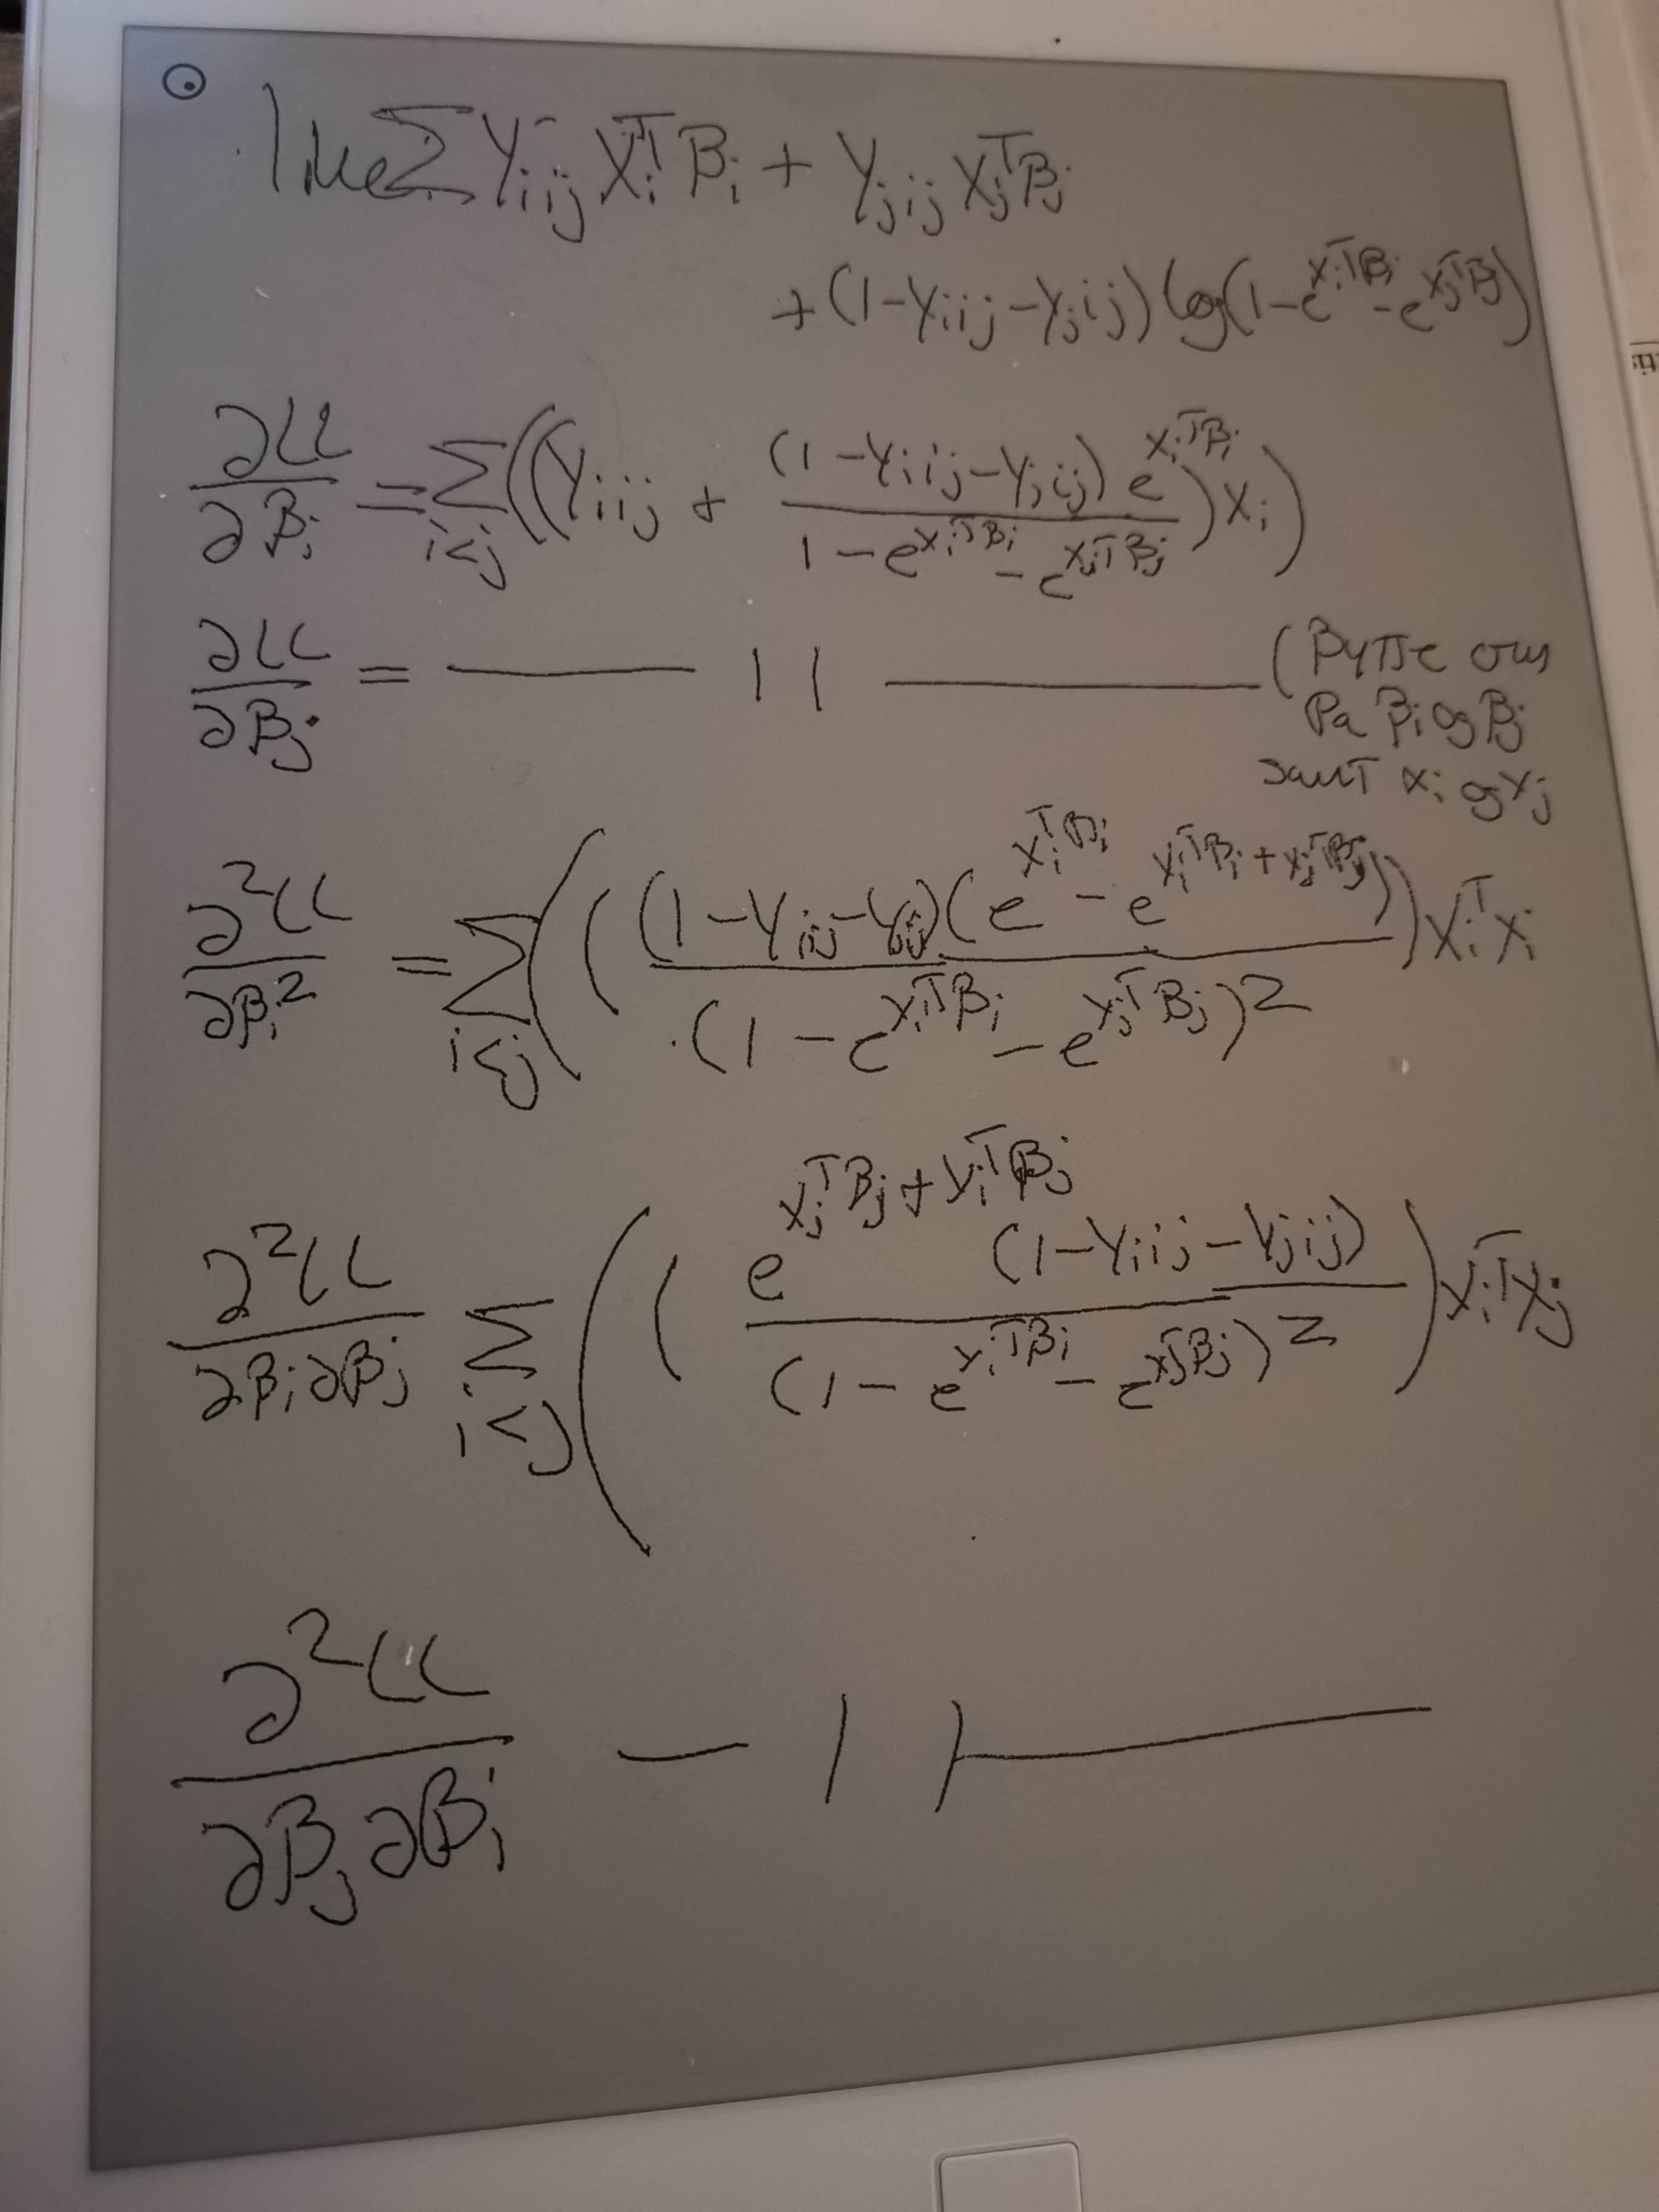
\includegraphics[scale=0.1]{ifmbt.jpg}
\end{center}

\textcolor{red}{
Til at beskrive disse sandsynligheder simultant vil det være oplagt at bruge multinomalfordelingen, og derfor definerer vi $n_{ij}$ til at være antal gange $i$ har 'vundet' over $j$, og $N_{ij}$ være antal gange $i$ og $j$ er blevet vurderet op imod hinanden. Eftersom der ofte vil være flere end to aktører der skal sammenlignes, definerer vi $t$ som værende antal aktører og $\{i,j\} \in \{i \neq j, 1 \leq i, j \leq t\}$. Derudover har vi at $N_{ij}$ er defineret af uafhængige sammenligninger med sandsynlighederne $\pi_{ij}$, kan $n_{ij}$ beskrives med en multinomialfordeling med antalsparameter $r = \sum_{i < j} N_{ij}$ og sandsynlighedsparametrene $\pi_{i\cdot ij},\pi_{j\cdot ij} \; og \; \pi_{0\cdot ij}$. \textcolor{blue}{Denne model kan beskrive parvise sandsynligheder for $2,...,l$ antal hold, og dermed $\binom{l}{2}$ uafhængige(?) sammenligninger, med $\binom{l}{2}$ - (l-1) frihedsgrader.} De parvise sammenligninger mellem $n_{ij} \ og \ n_{ji}$ kan ved hjælp af en kontingenstabel beskrives på formen:
}
$$
A = 
\begin{bmatrix}
&& Tabendehold &&
\\   
Vindendehold & H_1 & H_2 & H_3 & \cdots & H_l
\\ H_1 & - & n_{12} & n_{13} & \cdots & n_{1l} 
\\ H_2 & n_{21} & - & n_{23} & \cdots & n_{2l}
\\ H_3 & n_{31} & n_{32} & - & \cdots & n_{3l}
\\ \vdots & \vdots & \vdots & \vdots & - & \vdots
\\ H_l & n_{l1} &  n_{l2} & n_{l3} & \cdots & -
\end{bmatrix} 
$$

\subsection{Generel model med forskel på ude og hjemme}
Første mulighed, er at tilføje hjemmebanefordelen som en enkelt kategorisk variabel, når et hold spiller på hjemmebane. Denne vil symbolisere et gennemsnit af de forskellige klubbers hjemmebanefordel $\alpha$ (forøget sejrs succes når der spilles på hjemmebane). 
Eksempel a vinder over b, på a's hjemmebane. 
\begin{equation}
P(a\ vinder\ over\ b) = \frac{\beta_a}{\beta_a+\beta_b}+\alpha
\end{equation}

Vi kan også tilføje hjemmebanedelen, som et parameter for hver klub afhængigt af hvor godt de hver især performer på hjemmebane:
Det er samme princip, blot med t alpha parametre:
\begin{equation}
log(\frac{\Pi_{ab}}{\Pi_{ba}}) = \beta_a-\beta_b + \alpha_a
\end{equation}

Og tredje alternative model med $a$'s hjemmebaneeffekt som vekselvirkning:
\begin{equation}
P(a\ vinder\ over\ b) = \frac{\beta_a\alpha_a}{\beta_a\alpha_a+\beta_b}
\end{equation}
Denne parameter beskriver den hjemmebanefordel hold $a$ har. På denne måde kan man altså tilføje flere parametre til modellen, så det ikke længere kun er antal vundne kampe for hold $a \ og \ b$. Vi kan ikke antage en konstant hjemmebanefordel/effekt, da nogle hold kan have en stærkkere hjemmebane, og dermed vil $\alpha$ være forskellig for hvert hold $a$, hvor $\alpha_a>0$.
\\
\subsection{Udvidet model med flere udfald}
Den generelle model kan ifølge Rao and Kupper (1967) udvides til at have tre udfald, ved at tilføje et grænseværdi-parameter $\theta$, der fjerner betingelsen fra 1.1 med $\Pi_{ab}+\Pi_{ba}=1$ (på $a$'s hjemmebane). For nemhedens skyld noterer vi a vinder over b som 1, b vinder over a som 2 og a spiller uafgjort mod b som 3, samt Y som værende parameteren vi vil estimere for:

\begin{align*}
P(Y=1) &= \frac{\pi_i}{\pi_i+\pi_j\theta}\\
P(Y=2) &= \frac{\pi_j}{\pi_j+\pi_i\theta}\\
P(Y=3) &= \frac{\pi_i\pi_j(\theta^2-1)}{(\pi_i+\pi_j\theta)(\pi_i\theta+\pi_j)}
\end{align*}
Eftersom sandsynlighederne hver især skal opfylde:
$P(Y=1)>0, \ P(Y=2)>0\ og \ P(Y=3)>0\ samt P(Y=1)+P(Y=2)+P(Y=3)=1$, er det en nødvendig betingelse at $\theta>1$.
For at estimere disse sandsynligheder er det oplagt \textcolor{red}{(finde henvisning til at vi bruger en multinomial fordeling)} at bruge en multinomial fordeling, med de tre ovenstående sandsynligheder, med \textcolor{red}{(de stokastiske parametre?)} parametrene $\beta \ og \ \theta$. 

\subsection{Estimering af $\pi$ og $\theta$ }

Hvis vi definere, $s_{ij}$, $t_{ij}$ samt $u_{ij}$ for hhv. antal sejrer, tab og uafgjort for hold i mod hold j. Så kan vi i det enkelte tilfælde for den k'te kamp mellem hold i og j, opstille likelihooden som: 
\begin{align*}
\mathcal{L}_{ijk} &= \Big{(}\frac{\pi_i}{\pi_i+\theta\pi_j}\Big{)}^{s_{ijk}}
\;\Big{(}\frac{\pi_j}{\pi_j+\theta\pi_i}\Big{)}^{t_{ijk}}
\Big{(}\frac{(\theta^2-1)\pi_i \pi_j}{(\pi_i+\theta\pi_j)(\pi_j+\theta\pi_i)}\Big{)}^{u_{ijk}}\\
&= (\theta^2-1)^{u_{ijk}}\Big{(}\frac{\pi_i}{\pi_i+\theta\pi_j}\Big{)}^{SU_{ijk}}\Big{(}\frac{\pi_j}{\pi_j+\theta\pi_i}\big{)}^{SU_{jik}}
\end{align*}
Hvor, $S=\sum_{i<j}s_{ij}$,  $T=\sum_{i<j}t_{ij}$ og $U=\sum_{i<j}u_{ij}$ samt $SU_{ij}=\sum_{j(\neq i)}\big{(}s_{ij}+u_{ij}\big{)}$ \\
\\
Thi bliver likelihooden for alle observationer:
\begin{align*}
L(\pi_1,\pi_2,..,\pi_h;\theta) &=(\theta^2-1)^U\prod_i\pi_i^{SU_i}\prod_{i\neq j}\big{(}\pi_i+\theta\pi_j\big{)}^{-SU_{ij}}
\end{align*}
\\\\
Vi kan nu opstille log-likelihooden og tilføje en lagrange multiplikator for bibetingelsen\\ $\sum_i\pi_i=1$:
\begin{align*}
l(\pi_1,\pi_2,..,\pi_h;\theta) 
&=U\;log(\theta^2-1)+\sum_i SU_{i}\;log(\pi_i)-\sum_{i \neq j}SU_{ij}\;log\big{(}\pi_i+\theta \pi_j\big{)}-\lambda\big{(}\sum_i(\pi_i)-1\big{)}\\
\end{align*}
Log-likelihooden kan omskrives, hvor alle led der ikke indeholder $\pi_i$ fjernes, til:
$$l(\pi_i)=SU_i \; log(\pi_i) - \sum_{j(\neq i)}SU_{ij}\;log(\pi_i + \theta \pi_j) - \sum_{j(\neq i)} SU_{ji}\; log(\pi_j + \theta \pi_i)-\lambda \pi_i$$
\\
Vi kan nu opstille førsteordens betingelserne: 
\begin{equations}
\begin{align}
 \frac{\partial \ell(\pi;\theta)}{\partial \pi_i}&= 
\frac{SU_i}{\hat{\pi_i}}-\sum_{j(\neq i)}\frac{SU_{ij}}{\hat{\pi_i}+\theta \pi_j}-\sum_{j(\neq i)}\frac{\theta SU_{ji}}{\pi_j + \theta \hat{\pi_i}}-\lambda=0\\
\frac{\partial \ell(\pi;\theta)}{\partial \theta}&=
\frac{2U\hat{\theta}}{\hat{\theta}^2-1}-\sum_{i \neq j}\frac{SU_{ij}\pi_j}{\pi+\hat{\theta}\pi_j}=0\\
\frac{\partial \ell(\pi;\theta)}{\partial \lambda}&=
\sum_i(\pi_i)=1
\end{align}
\end{equations}

\textcolor{red}{
\begin{equation}
\frac{\partial \ell(\pi;\theta)}{\partial \pi_i}= 
\frac{SU_i}{\hat{\pi_i}}-\sum_{j(\neq i)}\frac{SU_{ij}}{\hat{\pi_i}+\theta \pi_j}-\sum_{j(\neq i)}\frac{\theta SU_{ji}}{\pi_j + \theta \hat{\pi_i}}-\lambda=0
\end{equation}
\begin{equation}
\frac{\partial \ell(\pi;\theta)}{\partial \theta}=
\frac{2U\hat{\theta}}{\hat{\theta}^2-1}-\sum_{i \neq j}\frac{SU_{ij}\pi_j}{\pi+\hat{\theta}\pi_j}=0
\end{equation}
\begin{equation}
\frac{\partial \ell(\pi;\theta)}{\partial \lambda}=\sum_i(\pi_i)=1
\end{equation}
}
Netwon-Raphson:
Initialiserer med\\ $x_{k} = x_0$\\
Opdaterer med:\\
$x_{k+1}=x_{k}-f'(x_{k})/f''(x_{k})$\\
Termination:\\
$|f(x_{k})|< tolerance$ med n-antal decimaler.
I n-dimensioner:\\
$
w_{k} = \left(
\begin{array}{c}
\pi_i\\
\theta
\end{array}
\right) 
$
$
\Delta=\left(
\begin{array}{c}
 \frac{\text{dl}}{\text{d$\pi $}_i} \\
 \frac{\text{dl}}{\text{d$\theta $}} \\
\end{array}
\right)
$
\\
$
H=\left(
\begin{array}{cc}
 \frac{\text{dl}}{d \pi _i \pi _i} & \frac{\text{dl}}{d   \pi _i \theta} \\
 \frac{\text{dl}}{d \theta  \pi _i} & \frac{\text{dl}}{d \theta \theta } \\
\end{array}
\right)
$
\\
$
w_{k+t}=w_k-H^{-1}\Delta
$
%################################################################
\section{Least Absolute Shrinkage and Selection Operator}

\section{Gammelt Lort}
\begin{equation}
log(\frac{\Pi_{ab}}{\Pi_{ba}}) = \beta_a-\beta_b
\end{equation}

Hvis vi definere, $s_{ij}$, $t_{ij}$ samt $u_{ij}$ for hhv. sejrer, tab og uafgjort for hold i. Så kan vi i det enkelte tilfælde for den k'te kamp mellem hold i og j, opstille Likelihooden som: 

$$
\mathcal{L}_{ijk}=\Big{(}\frac{\pi_i}{\pi_i+\theta\pi_j}\Big{)}^{s_{ijk}}
\;\Big{(}\frac{\pi_j}{\pi_j+\theta\pi_i}\Big{)}^{t_{ijk}}
\Big{(}\frac{(\theta^2-1)\pi_i \pi_j}{(\pi_i+\theta\pi_j)(\pi_j+\theta\pi_i)}\Big{)}^{u_{ijk}}
\;
$$
Thi bliver likilihooden for de samlede observationer mellem de h antal hold:
$$
\mathcal{L}(\pi_1,\pi_2,..,\pi_h;\theta)=\binom{n}{S\;T\;U}\prod_{i=1}\prod_{j=1}\Big{(}\frac{\pi_i}{\pi_i+\theta\pi_j}\Big{)}^{s_{ij}}
\;\textcolor{red}{\Big{(}\frac{\pi_j}{\pi_j+\theta\pi_i}\Big{)}^{t_{ij}}}
\Big{(}\frac{(\theta^2-1)\pi_i \pi_j}{(\pi_i+\theta\pi_j)(\pi_j+\theta\pi_i)}\Big{)}^{\frac{1}{2}u_{ij}}
$$
Likelihood funktionen kan opskrives som nedenstående, hvor $s_{ij}$ viser antal vundne kampe for $i$ mod $j$ og $u_{ij}$ er antal uafgjorte for $i$ mod $j$. Eftersom vi itererer over både $i$ og $j$ vil de uafgjorte kampe blive fordoblet, hvorfor der ganges med en halv i potensen. 
$$
\mathcal{L}(\pi_1,\pi_2,..,\pi_h;\theta)=\binom{n}{S\;T\;U}\prod_{i=1}\prod_{j=1}\Big{(}\frac{\pi_i}{\pi_i+\theta\pi_j}\Big{)}^{s_{ij}}
\Big{(}\frac{(\theta^2-1)\pi_i \pi_j}{(\pi_i+\theta\pi_j)(\pi_j+\theta\pi_i)}\Big{)}^{\frac{1}{2}u_{ij}}
\;
$$
Hvor r, er antal kampe mellem hold i og j samt $S=\sum_{i<j}s_{ij}$,  $T=\sum_{i<j}t_{ij}$ og $U=\sum_{i<j}u_{ij}$
\\
\textcolor{red}{Er usikker på, om vi blot skal finde MLE for $\pi_i$ eller begge? vi har vel kun hold i mod j og ikke hold j mod i?}
\\
$$
\ell(\pi_1,\pi_2,..,\pi_h;\theta)=\sum_{i=1}\sum_{j=1}\Big{[}s_{ij}\;Log\Big{(}\frac{\pi_i}{\pi_i+\theta\pi_j}\Big{)}+
\frac{1}{2}u_{ij}\;Log\Big{(}\frac{(\theta^2-1)\pi_i \pi_j}{(\pi_i+\theta\pi_j)(\pi_j+\theta\pi_i)}\Big{)}\Big{]}
\;
$$

Ved at opstille første ordens betingelserne $\frac{\partial \ell(\pi;\theta)}{\partial \pi_i}=0$, 
\textcolor{red}{Da $\pi_i$ antager alle hold, burde det ikke være nødvendigt med denne
$\frac{\partial \ell(\pi;\theta)}{\partial \pi_j}=0$} samt $\frac{\partial \ell(\pi;\theta)}{\partial \theta}=0$ kan vi nu løse ligningsystemerne og finde vores maksimum likelihood estimater $\hat{\pi_i}$ og $\hat{\theta}$ for hhv. $\pi_i(i=1,2,...,h)$ og $\theta$. 

\begin{equation}
\frac{\partial \ell(\pi;\theta)}{\partial \pi_i}=\sum_i\sum_j \frac{s_{ij}+\frac{1}{2}u_{ij}}{\pi_i}-\frac{s_{ij}+\frac{1}{2}u_{ij}}{\pi_i+\theta\pi_j}-\frac{\theta\frac{1}{2}u_{ij}}{\pi_j+\theta\pi_i}=0
\end{equation}

\begin{equation}
\frac{\partial \ell(\pi;\theta)}{\partial \theta}=\sum_i\sum_j
\frac{\theta u_{ij}}{\theta^2-1}
- \frac{\pi_j(s_{ij}+\frac{1}{2}u_{ij})}{\pi_i+\theta \pi_j}
- \frac{\frac{1}{2}u_{ij}\pi_i}{\pi_j+\theta \pi_i}=0
\end{equation}

\newpage
\subsection{Fra BradleyTerry2}
\begin{lstlisting}
#Funktion til at estimeere BT for to udfald..
function (outcome = 1, player1, player2, formula = NULL, id = "..", 
    separate.ability = NULL, refcat = NULL, family = "binomial", 
    data = NULL, weights = NULL, subset = NULL, na.action = NULL, 
    start = NULL, etastart = NULL, mustart = NULL, offset = NULL, 
    br = FALSE, model = TRUE, x = FALSE, contrasts = NULL, ...) 
{
    call <- match.call()
    if (is.character(family)) 
        family <- get(family, mode = "function", envir = parent.frame())
    if (is.function(family)) 
        family <- family()
    if (is.null(family$family)) {
        print(family)
        stop("`family' not recognized")
    }
    if (family$family != "binomial") 
        stop("`family' must be binomial")
    if (!family$link %in% c("logit", "probit", "cauchit")) 
        stop("link for binomial family must be one of \"logit\", \"probit\"", 
            "or \"cauchit\"")
    fcall <- as.list(match.call(expand.dots = FALSE))
    if (is.null(formula)) {
        formula <- reformulate(id)
        environment(formula) <- parent.frame()
        fcall$formula <- formula
    }
    setup <- match(c("outcome", "player1", "player2", "formula", 
        "id", "separate.ability", "refcat", "data", "weights", 
        "subset", "offset", "contrasts"), names(fcall), 0L)
    setup <- do.call(BTm.setup, fcall[setup], envir = parent.frame())
    if (setup$saturated) 
        warning("Player ability saturated - equivalent to fitting ", 
            "separate abilities.")
    mf <- data.frame(X = setup$player1)
    if (!is.null(setup$X)) {
        mf$X <- setup$X
        formula <- Y ~ X - 1
    }
    else formula <- Y ~ 0
    mf$Y <- setup$Y
    argPos <- match(c("na.action", "start", "etastart", "mustart", 
        "control", "model", "x"), names(fcall), 0)
    dotArgs <- fcall$...
    if (is.null(setup$random)) {
        method <- get(ifelse(br, "brglm", "glm"), mode = "function")
        fit <- as.call(c(method, fcall[argPos], list(formula = formula, 
            family = family, data = mf, offset = setup$offset, 
            subset = setup$subset, weights = setup$weights), 
            dotArgs))
        fit <- eval(fit, parent.frame())
    }
    else {
        method <- get("glmmPQL", mode = "function")
        fit <- as.call(c(method, fcall[argPos], list(formula, 
            setup$random, family = family, data = mf, offset = setup$offset, 
            subset = setup$subset, weights = setup$weights), 
            dotArgs))
        fit <- eval(fit, parent.frame())
        if (br) {
            if (identical(fit$sigma, 0)) {
                argPos <- match(c("na.action", "model", "x"), 
                  names(fcall), 0)
                method <- get("brglm", mode = "function")
                fit <- as.call(c(method, fcall[argPos], list(formula, 
                  family = family, data = mf, offset = setup$offset, 
                  subset = setup$subset, weights = setup$weights, 
                  etastart = fit$linear.predictors)))
                fit <- eval(fit, parent.frame())
                fit$class <- c("glmmPQL", class(fit))
            }
            else warning("'br' argument ignored for models with random effects", 
                call. = FALSE)
        }
    }
    if (length(fit$coefficients)) {
        if (ncol(setup$X) > 1) 
            names(fit$coefficients) <- substring(names(fit$coefficients), 
                2)
        else names(fit$coefficients) <- colnames(setup$X)
        fit$assign <- attr(setup$X, "assign")
    }
    fit$call <- call
    fit$id <- id
    fit$separate.ability <- separate.ability
    fit$contrasts <- setup$contrasts
    fit$refcat <- setup$refcat
    fit$formula <- setup$formula
    fit$player1 <- setup$player1
    fit$player2 <- setup$player2
    fit$term.labels <- setup$term.labels
    fit$data <- setup$data
    fit$random <- setup$random
    class(fit) <- c("BTm", class(fit))
    fit
}
\end{lstlisting}

\end{document}